\documentclass[]{apa6}

\usepackage{amssymb,amsmath}
\usepackage{ifxetex,ifluatex}
\usepackage{fixltx2e} % provides \textsubscript
\ifnum 0\ifxetex 1\fi\ifluatex 1\fi=0 % if pdftex
  \usepackage[T1]{fontenc}
  \usepackage[utf8]{inputenc}
\else % if luatex or xelatex
  \ifxetex
    \usepackage{mathspec}
    \usepackage{xltxtra,xunicode}
  \else
    \usepackage{fontspec}
  \fi
  \defaultfontfeatures{Mapping=tex-text,Scale=MatchLowercase}
  \newcommand{\euro}{€}
\fi
% use upquote if available, for straight quotes in verbatim environments
\IfFileExists{upquote.sty}{\usepackage{upquote}}{}
% use microtype if available
\IfFileExists{microtype.sty}{\usepackage{microtype}}{}

% Table formatting
\usepackage{longtable, booktabs}
\usepackage{lscape}
% \usepackage[counterclockwise]{rotating}   % Landscape page setup for large tables
\usepackage{multirow}		% Table styling
\usepackage{tabularx}		% Control Column width
\usepackage[flushleft]{threeparttable}	% Allows for three part tables with a specified notes section
\usepackage{threeparttablex}            % Lets threeparttable work with longtable

% Create new environments so endfloat can handle them
% \newenvironment{ltable}
%   {\begin{landscape}\begin{center}\begin{threeparttable}}
%   {\end{threeparttable}\end{center}\end{landscape}}

\newenvironment{lltable}
  {\begin{landscape}\begin{center}\begin{ThreePartTable}}
  {\end{ThreePartTable}\end{center}\end{landscape}}

  \usepackage{ifthen} % Only add declarations when endfloat package is loaded
  \ifthenelse{\equal{\string }{\string man}}{%
   \DeclareDelayedFloatFlavor{ThreePartTable}{table} % Make endfloat play with longtable
   % \DeclareDelayedFloatFlavor{ltable}{table} % Make endfloat play with lscape
   \DeclareDelayedFloatFlavor{lltable}{table} % Make endfloat play with lscape & longtable
  }{}%



% The following enables adjusting longtable caption width to table width
% Solution found at http://golatex.de/longtable-mit-caption-so-breit-wie-die-tabelle-t15767.html
\makeatletter
\newcommand\LastLTentrywidth{1em}
\newlength\longtablewidth
\setlength{\longtablewidth}{1in}
\newcommand\getlongtablewidth{%
 \begingroup
  \ifcsname LT@\roman{LT@tables}\endcsname
  \global\longtablewidth=0pt
  \renewcommand\LT@entry[2]{\global\advance\longtablewidth by ##2\relax\gdef\LastLTentrywidth{##2}}%
  \@nameuse{LT@\roman{LT@tables}}%
  \fi
\endgroup}


  \usepackage{graphicx}
  \makeatletter
  \def\maxwidth{\ifdim\Gin@nat@width>\linewidth\linewidth\else\Gin@nat@width\fi}
  \def\maxheight{\ifdim\Gin@nat@height>\textheight\textheight\else\Gin@nat@height\fi}
  \makeatother
  % Scale images if necessary, so that they will not overflow the page
  % margins by default, and it is still possible to overwrite the defaults
  % using explicit options in \includegraphics[width, height, ...]{}
  \setkeys{Gin}{width=\maxwidth,height=\maxheight,keepaspectratio}
\ifxetex
  \usepackage[setpagesize=false, % page size defined by xetex
              unicode=false, % unicode breaks when used with xetex
              xetex]{hyperref}
\else
  \usepackage[unicode=true]{hyperref}
\fi
\hypersetup{breaklinks=true,
            pdfauthor={},
            pdftitle={The title},
            colorlinks=true,
            citecolor=blue,
            urlcolor=blue,
            linkcolor=black,
            pdfborder={0 0 0}}
\urlstyle{same}  % don't use monospace font for urls

\setlength{\parindent}{0pt}
%\setlength{\parskip}{0pt plus 0pt minus 0pt}

\setlength{\emergencystretch}{3em}  % prevent overfull lines


% Manuscript styling
\captionsetup{font=singlespacing,justification=justified}
\usepackage{csquotes}
\usepackage{upgreek}



\usepackage{tikz} % Variable definition to generate author note

% fix for \tightlist problem in pandoc 1.14
\providecommand{\tightlist}{%
  \setlength{\itemsep}{0pt}\setlength{\parskip}{0pt}}

% Essential manuscript parts
  \title{The title}

  \shorttitle{Title}


  \author{First Author\textsuperscript{1}~\& Ernst-August Doelle\textsuperscript{1,2}}

  % \def\affdep{{"", ""}}%
  % \def\affcity{{"", ""}}%

  \affiliation{
    \vspace{0.5cm}
          \textsuperscript{1} Wilhelm-Wundt-University\\
          \textsuperscript{2} Konstanz Business School  }

  \authornote{
    Correspondence concerning this article should be addressed to First
    Author, Postal address. E-mail:
    \href{mailto:my@email.com}{\nolinkurl{my@email.com}}
  }


  \abstract{One or two sentences providing a \textbf{basic introduction} to the
field, comprehensible to a scientist in any discipline.

Two to three sentences of \textbf{more detailed background},
comprehensible to scientists in related disciplines.

One sentence clearly stating the \textbf{general problem} being
addressed by this particular study.

One sentence summarizing the main result (with the words ``\textbf{here
we show}'' or their equivalent).

Two or three sentences explaining what the \textbf{main result} reveals
in direct comparison to what was thought to be the case previously, or
how the main result adds to previous knowledge.

One or two sentences to put the results into a more \textbf{general
context}.

Two or three sentences to provide a \textbf{broader perspective},
readily comprehensible to a scientist in any discipline.}
  \keywords{keywords \\

    \indent Word count: X
  }





\usepackage{amsthm}
\newtheorem{theorem}{Theorem}[section]
\newtheorem{lemma}{Lemma}[section]
\theoremstyle{definition}
\newtheorem{definition}{Definition}[section]
\newtheorem{corollary}{Corollary}[section]
\newtheorem{proposition}{Proposition}[section]
\theoremstyle{definition}
\newtheorem{example}{Example}[section]
\theoremstyle{definition}
\newtheorem{exercise}{Exercise}[section]
\theoremstyle{remark}
\newtheorem*{remark}{Remark}
\newtheorem*{solution}{Solution}
\begin{document}

\maketitle

\setcounter{secnumdepth}{0}



\section{CCS Concepts}\label{ccs-concepts}

Applied computing \textasciitilde{} Education \textasciitilde{} Learning
management systems Applied computing \textasciitilde{} Education
\textasciitilde{} E-learning Applied computing \textasciitilde{}
Education \textasciitilde{} Computer-managed instruction

\section{Keywords}\label{keywords}

\section{1. INTRODUCTION}\label{introduction}

In recent years, educational institutions have begun to collect student
data (REF). One area of interest is the delivery of fully online
instruction, which is becoming more prevalent (REF). Specifically,
online education is available for K-12 students who cannot or prefer not
to attend a brick-and-mortar school (REF). We seek to examine in the
current study the educational experiences of students in online science
courses at a virtual middle school.

One meaningful perspective from which to consider students' engagement
with online courses is related to their motivation to achieve. More
specifically, it is important to consider how and why students are
engaging with the course. To consider the psychological mechanisms
behind achievement is valuable because doing so may help to identify
meaningful points of intervention for educators.

Expectancy-value theory (EVT) is a key motivational framework that
explains the reasons that students are motivated to achieve (Eccles et
al., 1983). EVT posits that students are motivated to achieve when (1)
they perceive themselves to be capable of success (e.g.,
\enquote{expectancy}) and (2) they perceive present or future value in
the task at hand (e.g., \enquote{value}). Two types of value are utility
value, which refers to the degree to which students perceive that a
given task will be useful to them for some future goal, and interest
value, which refers to the level of interest students have in a given
task. In this study, we will consider utility value, interest value, and
expectancy for success as predictors of student achievement.

We are fortunate to have a robust dataset which includes self-reported
motivation as well as behavioral trace data which was collected from the
learning management system. (MAYBE SAY MORE ABOUT THIS IN THE METHOD
INSTEAD OF INTRO\ldots{}? - EAB 9.21.2018)

We investigated three research questions: (1) Is motivation -
operationalized as interest value, utility value and perceived
competence for science - relatively more predictive of course grades as
compared to other online indicators of engagement? (2) Which types of
motivation (e.g., interest value, utility value, and perceived
competence) is most predictive of achievement? (3) Which types of trace
measures (e.g.,\\
- cogproc - social - posemo - negemo - perscon - n (this is the number
of posts) are most predictive?

\subsection{Notes on Intro from the
call}\label{notes-on-intro-from-the-call}

We welcome theoretical, methodological, empirical and technical
contributions to all fields related to learning analytics. Related to
our special theme the following topics are of particular interest:

\begin{itemize}
\tightlist
\item
  Universal design for learning promotes an inclusive approach to the
  curriculum -- how can learning analytics support curriculum design and
  revision from this perspective?
\item
  How can analytics be applied in ways that support inclusion and
  success?
\item
  How can the training of data scientists be made more inclusive?
\item
  What does educational success look like, and how can it be supported?
\item
  How can systematic biases (e.g.~related to diversity) in our analytics
  algorithms be identified, reflected, and possibly avoided?
\end{itemize}

\section{A. BACKGROUND AND RELATED
WORK}\label{a.-background-and-related-work}

! We might not need this section, I got the idea from a full paper. I
think it overlaps with intro

\section{2. METHOD}\label{method}

\subsection{2.1 Participants}\label{participants}

Participants were \#\#\#\#\#\# students enrolled in online middle school
science courses in \_\_\_\_years\_\_\_\_.

\subsection{2.2 Setting / Data Sources}\label{setting-data-sources}

\subsection{2.3 Procedure}\label{procedure}

\subsection{2.4 Data analysis}\label{data-analysis}

We used R (Version 3.5.1; R Core Team, 2017) and the R-package
\emph{papaja} (Version 0.1.0.9709; Aust \& Barth, 2018) for all our
analyses.

For our analyses, we used

\section{3. RESULTS}\label{results}

\begin{verbatim}
## Skim summary statistics
##  n obs: 662 
##  n variables: 111 
## 
## -- Variable type:character -----------------------------------------------------------
##           variable missing complete   n min max empty n_unique
##          course_ID       0      662 662  12  13     0       36
##  enrollment_reason       2      660 662   5  34     0        5
##  enrollment_status       2      660 662   7  17     0        3
##            section       0      662 662   2   2     0        4
##           semester       0      662 662   4   4     0        4
##            subject       0      662 662   4   5     0        5
## 
## -- Variable type:integer -------------------------------------------------------------
##  variable missing complete   n  mean    sd p0 p25 p50 p75 p100     hist
##         n     133      529 662 22.59 11.98  1  14  21  33   55 ▅▅▇▆▂▆▁▁
## 
## -- Variable type:numeric -------------------------------------------------------------
##      variable missing complete   n       mean        sd       p0
##       achieve     133      529 662     1.1        0.67      0   
##           adj     133      529 662     4.72       1.4       0   
##        adverb     133      529 662     6.15       1.76      0   
##        affect     133      529 662     6.11       2.12      0   
##   affiliation     133      529 662     1.46       1.02      0   
##       AllPunc     133      529 662    13.15       4.14      0   
##      Analytic     133      529 662    52.87      12.33      6.64
##         anger     133      529 662     0.16       0.2       0   
##           anx     133      529 662     0.16       0.26      0   
##       Apostro     133      529 662     1.18       0.99      0   
##       article     133      529 662     6.92       1.68      0   
##        assent     133      529 662     0.87       1.27      0   
##     Authentic     133      529 662    42.87      13.16      1   
##       auxverb     133      529 662     9.22       1.86      0   
##           bio     133      529 662     2.75       2         0   
##          body     133      529 662     1.45       1.8       0   
##         cause     133      529 662     2.79       1.31      0   
##       certain     133      529 662     1.49       0.75      0   
##         Clout     133      529 662    50.02      11.08      5.06
##       cogproc     133      529 662    13.92       3.5       0   
##         Colon     133      529 662     0.12       0.29      0   
##         Comma     133      529 662     2.84       1.56      0   
##       compare     133      529 662     2.45       0.89      0   
##          conj     133      529 662     6.53       1.53      0   
##          Dash     133      529 662     0.38       0.94      0   
##         death     133      529 662     0.097      0.12      0   
##           Dic     133      529 662    83.3        6.74      0   
##        differ     133      529 662     2.93       1.16      0   
##       discrep     133      529 662     1.64       0.84      0   
##        drives     133      529 662     5.81       1.84      0   
##        Exclam     133      529 662     1.4        2.13      0   
##        family     133      529 662     0.12       0.27      0   
##          feel     133      529 662     0.85       0.66      0   
##        female     133      529 662     0.14       0.28      0   
##        filler     133      529 662     0.0059     0.026     0   
##   final_grade      28      634 662    77.37      21.44      0.9 
##   focusfuture     133      529 662     0.71       0.5       0   
##     focuspast     133      529 662     3.29       1.64      0   
##  focuspresent     133      529 662    10.6        2.18      0   
##        friend     133      529 662     0.099      0.21      0   
##      function     133      529 662    51.87       5.28      0   
##        health     133      529 662     1.01       0.81      0   
##          hear     133      529 662     0.34       0.36      0   
##          home     133      529 662     0.21       0.34      0   
##             i     133      529 662     4.74       2.06      0   
##      informal     133      529 662     1.41       1.48      0   
##        ingest     133      529 662     0.37       0.47      0   
##       insight     133      529 662     3.9        1.53      0   
##      interrog     133      529 662     1.71       0.8       0   
##         ipron     133      529 662     6.47       1.77      0   
##       leisure     133      529 662     1.07       0.97      0   
##          male     133      529 662     0.24       0.29      0   
##         money     133      529 662     0.32       0.34      0   
##        motion     133      529 662     1.34       0.77      0   
##        negate     133      529 662     1.05       0.63      0   
##        negemo     133      529 662     0.87       0.61      0   
##      netspeak     133      529 662     0.19       0.46      0   
##        nonflu     133      529 662     0.25       0.41      0   
##        number     133      529 662     1.23       0.74      0   
##        OtherP     133      529 662     0.66       1.71      0   
##       Parenth     133      529 662     0.22       0.41      0   
##       percept     133      529 662     2.36       1.17      0   
##        Period     133      529 662     5.68       1.67      0   
##        posemo     133      529 662     5.22       2.07      0   
##      post_int     567       95 662     3.88       0.94      1   
##  post_percomp     567       95 662     3.47       0.88      1   
##       post_tv     567       95 662     3.71       0.9       1   
##       post_uv     567       95 662     3.48       0.99      1   
##         power     133      529 662     1.79       0.84      0   
##         ppron     133      529 662     8.31       2.18      0   
##       pre_int      12      650 662     4.3        0.6       1.8 
##   pre_percomp       7      655 662     3.64       0.69      1.5 
##        pre_tv      11      651 662     4.07       0.59      1   
##        pre_uv       6      656 662     3.75       0.75      1   
##          prep     133      529 662    11.55       1.96      0   
##       pronoun     133      529 662    14.79       2.81      0   
##         QMark     133      529 662     0.44       0.59      0   
##         quant     133      529 662     2.19       0.79      0   
##         Quote     133      529 662     0.019      0.067     0   
##       relativ     133      529 662     9.52       2.39      0   
##         relig     133      529 662     0.043      0.17      0   
##        reward     133      529 662     1.55       1.03      0   
##          risk     133      529 662     0.34       0.33      0   
##           sad     133      529 662     0.15       0.24      0   
##           see     133      529 662     1.06       0.75      0   
##         SemiC     133      529 662     0.22       0.45      0   
##        sexual     133      529 662     0.024      0.063     0   
##         shehe     133      529 662     0.25       0.28      0   
##        Sixltr     133      529 662    17.77       3.35      0   
##        social     133      529 662     6.54       1.86      0   
##         space     133      529 662     5.6        1.57      0   
##    student_ID       0      662 662 89347.69   12951.25  43146   
##         swear     133      529 662     0.0088     0.047     0   
##        tentat     133      529 662     2.62       1.25      0   
##          they     133      529 662     0.76       0.6       0   
##          time     133      529 662     2.62       1.12      0   
##    time_spent       3      659 662  1828.16    1358.82      0.45
##          Tone     133      529 662    67.05      11.81     11.04
##          verb     133      529 662    15.85       2.65      0   
##            WC     133      529 662    66.44      24.7       1   
##            we     133      529 662     0.5        0.59      0   
##          work     133      529 662     3.18       1.65      0   
##           WPS     133      529 662    15.95       4.07      1   
##           you     133      529 662     2.07       1.25      0   
##         p25        p50      p75      p100     hist
##      0.72       0.99       1.36      5.71 ▃▇▂▁▁▁▁▁
##      3.91       4.64       5.46     11.76 ▁▁▆▇▂▁▁▁
##      5.1        6.21       7.14     12.65 ▁▁▃▇▇▂▁▁
##      4.86       5.73       6.94     19.01 ▁▃▇▂▁▁▁▁
##      0.87       1.31       1.85      8.71 ▇▇▂▁▁▁▁▁
##     10.78      12.62      15.06     57.64 ▁▇▃▁▁▁▁▁
##     45.89      53.61      60.87     96.31 ▁▁▂▇▇▃▁▁
##      0          0.083      0.24      1.64 ▇▂▁▁▁▁▁▁
##      0          0.095      0.22      4.17 ▇▁▁▁▁▁▁▁
##      0.45       1.01       1.59      8.1  ▇▆▂▁▁▁▁▁
##      6.13       6.98       7.81     16.51 ▁▁▃▇▂▁▁▁
##      0.34       0.68       1.13     25    ▇▁▁▁▁▁▁▁
##     34.99      41.9       48.51     96.82 ▁▁▅▇▃▁▁▁
##      8.08       9.3       10.27     16.7  ▁▁▁▃▇▃▁▁
##      1.46       2.05       3.27     11.21 ▃▇▁▁▂▁▁▁
##      0.27       0.71       1.5      10.28 ▇▁▁▁▁▁▁▁
##      2          2.57       3.38     10.81 ▂▇▅▂▁▁▁▁
##      0.99       1.45       1.89      5.5  ▃▇▇▃▁▁▁▁
##     42.99      50.84      57.83     86.02 ▁▁▁▅▇▆▁▁
##     11.7       14.2       16.12     34.29 ▁▁▅▇▂▁▁▁
##      0          0.0054     0.1       3.66 ▇▁▁▁▁▁▁▁
##      1.7        2.64       3.69      9.52 ▃▇▇▅▂▁▁▁
##      1.87       2.37       3.01      5.34 ▁▂▇▇▆▃▁▁
##      5.63       6.44       7.36     17.41 ▁▁▇▇▁▁▁▁
##      0.0059     0.15       0.45     17.72 ▇▁▁▁▁▁▁▁
##      0          0.056      0.14      0.74 ▇▃▁▁▁▁▁▁
##     81.01      84.18      86.96     94.59 ▁▁▁▁▁▁▃▇
##      2.2        2.92       3.57      8.57 ▁▅▇▆▂▁▁▁
##      1.1        1.54       2.07      8.57 ▃▇▃▁▁▁▁▁
##      4.61       5.48       6.71     16.22 ▁▂▇▃▂▁▁▁
##      0.14       0.79       1.96     31.44 ▇▁▁▁▁▁▁▁
##      0          0.056      0.15      4.89 ▇▁▁▁▁▁▁▁
##      0.45       0.76       1.14      7.48 ▇▅▁▁▁▁▁▁
##      0          0.066      0.19      4.89 ▇▁▁▁▁▁▁▁
##      0          0          0         0.26 ▇▁▁▁▁▁▁▁
##     71.07      83.69      91.87    100    ▁▁▁▁▁▃▆▇
##      0.36       0.61       0.93      2.86 ▆▇▅▂▁▁▁▁
##      2.08       3.09       4.48      9.81 ▂▇▇▆▅▁▁▁
##      9.17      10.63      11.86     19.52 ▁▁▁▅▇▃▁▁
##      0          0.029      0.11      2.22 ▇▁▁▁▁▁▁▁
##     49.61      52.41      54.99     64.86 ▁▁▁▁▁▂▇▂
##      0.47       0.81       1.38      4.88 ▇▇▃▂▁▁▁▁
##      0.098      0.25       0.47      3.33 ▇▂▁▁▁▁▁▁
##      0          0.13       0.3       5.5  ▇▁▁▁▁▁▁▁
##      3.55       4.38       5.36     16.67 ▁▇▇▁▁▁▁▁
##      0.76       1.19       1.8      27.27 ▇▁▁▁▁▁▁▁
##      0.037      0.2        0.51      3.78 ▇▂▁▁▁▁▁▁
##      2.78       3.91       4.88     12    ▁▅▇▆▁▁▁▁
##      1.22       1.65       2.13      6.73 ▂▇▆▂▁▁▁▁
##      5.36       6.45       7.54     17.91 ▁▂▇▆▁▁▁▁
##      0.54       0.87       1.34      8.49 ▇▃▁▁▁▁▁▁
##      0          0.15       0.37      1.69 ▇▃▂▁▁▁▁▁
##      0.067      0.25       0.47      3.03 ▇▃▁▁▁▁▁▁
##      0.86       1.27       1.69      6.67 ▃▇▃▁▁▁▁▁
##      0.62       0.97       1.39      3.92 ▃▇▆▃▁▁▁▁
##      0.51       0.78       1.15      6.43 ▇▆▁▁▁▁▁▁
##      0          0.035      0.21      4.76 ▇▁▁▁▁▁▁▁
##      0          0.13       0.35      3.6  ▇▁▁▁▁▁▁▁
##      0.78       1.14       1.54      6.78 ▅▇▃▁▁▁▁▁
##      0.07       0.32       0.79     34.55 ▇▁▁▁▁▁▁▁
##      0          0.057      0.26      3.79 ▇▁▁▁▁▁▁▁
##      1.6        2.35       2.89     14.02 ▃▇▁▁▁▁▁▁
##      4.68       5.56       6.71     12.9  ▁▁▅▇▅▁▁▁
##      4.02       4.92       6        19.01 ▁▇▇▂▁▁▁▁
##      3.5        4          4.5       5    ▁▁▁▃▁▇▅▆
##      3          3.5        4         5    ▂▁▃▅▇▇▂▂
##      3.29       3.86       4.29      5    ▁▂▂▃▅▇▇▇
##      3          3.67       4         5    ▁▂▁▃▂▇▂▃
##      1.25       1.64       2.16      5.78 ▁▇▇▃▁▁▁▁
##      6.95       8.14       9.42     17.3  ▁▁▃▇▆▂▁▁
##      4          4.4        4.8       5    ▁▁▁▁▃▆▅▇
##      3          3.5        4         5    ▁▁▂▆▇▇▅▂
##      3.71       4.12       4.46      5    ▁▁▁▁▂▇▆▆
##      3.33       3.67       4.33      5    ▁▁▁▃▃▇▂▃
##     10.51      11.7       12.68     18.76 ▁▁▁▂▇▇▁▁
##     12.94      14.81      16.32     26.19 ▁▁▁▅▇▃▁▁
##      0          0.23       0.64      4.88 ▇▂▁▁▁▁▁▁
##      1.74       2.17       2.66      5.14 ▁▂▇▇▅▂▁▁
##      0          0          0         0.78 ▇▁▁▁▁▁▁▁
##      8.16       9.34      10.93     20.91 ▁▁▂▇▃▁▁▁
##      0          0          0         2.54 ▇▁▁▁▁▁▁▁
##      0.92       1.36       1.99      9.76 ▇▇▂▁▁▁▁▁
##      0.088      0.26       0.51      2.36 ▇▃▂▁▁▁▁▁
##      0          0.073      0.19      2.86 ▇▁▁▁▁▁▁▁
##      0.54       1.03       1.41      5.66 ▆▇▃▁▁▁▁▁
##      0          0.1        0.27      7.88 ▇▁▁▁▁▁▁▁
##      0          0          0.02      0.56 ▇▁▁▁▁▁▁▁
##      0          0.16       0.38      1.4  ▇▃▂▁▁▁▁▁
##     16.05      17.76      19.8      26.19 ▁▁▁▁▅▇▃▁
##      5.38       6.42       7.55     17.45 ▁▂▇▇▂▁▁▁
##      4.61       5.5        6.44     12.5  ▁▁▅▇▃▁▁▁
##  85935.75   89450      95482.75 115888    ▁▁▁▁▆▇▁▂
##      0          0          0         0.61 ▇▁▁▁▁▁▁▁
##      1.9        2.52       3.1      17.14 ▅▇▁▁▁▁▁▁
##      0.33       0.67       1.07      3.4  ▇▇▆▂▁▁▁▁
##      2          2.57       3.06      9.4  ▁▆▇▂▁▁▁▁
##    902.59    1551.35    2414.9    8870.88 ▇▇▃▂▁▁▁▁
##     60.59      67.4       73.38     99    ▁▁▁▂▆▇▂▁
##     14.37      15.97      17.55     23.67 ▁▁▁▁▅▇▃▁
##     51.33      61.68      79.58    234.92 ▁▇▇▂▁▁▁▁
##      0.13       0.34       0.73      8.11 ▇▁▁▁▁▁▁▁
##      2.22       3          3.82     14.67 ▂▇▃▁▁▁▁▁
##     13.37      15.55      18.13     44.5  ▁▂▇▃▁▁▁▁
##      1.19       1.98       2.71      6.58 ▅▆▇▃▃▁▁▁
\end{verbatim}

\begin{verbatim}
## Skim summary statistics
##  n obs: 499 
##  n variables: 16 
## 
## -- Variable type:character -----------------------------------------------------------
##           variable missing complete   n min max empty n_unique
##          course_ID       0      499 499  12  13     0       25
##  enrollment_reason       0      499 499   5  34     0        5
##  enrollment_status       0      499 499  17  17     0        1
##           semester       0      499 499   4   4     0        3
##            subject       0      499 499   4   5     0        5
## 
## -- Variable type:integer -------------------------------------------------------------
##  variable missing complete   n  mean    sd p0  p25 p50 p75 p100     hist
##         n       0      499 499 23.27 11.65  1 15.5  22  34   55 ▃▅▇▆▂▆▁▁
## 
## -- Variable type:numeric -------------------------------------------------------------
##     variable missing complete   n    mean      sd   p0    p25     p50
##      cogproc       0      499 499   14.03    3.41 0     11.87   14.32
##  final_grade       0      499 499   78.26   20.7  2.93  71.67   84.99
##       negemo       0      499 499    0.87    0.59 0      0.52    0.79
##       posemo       0      499 499    5.2     2.01 0      4.02    4.9 
##      pre_int       0      499 499    4.28    0.6  1.8    4       4.4 
##  pre_percomp       0      499 499    3.62    0.69 2      3       3.5 
##       pre_uv       0      499 499    3.76    0.75 1      3.33    3.67
##       social       0      499 499    6.49    1.75 0      5.38    6.36
##   time_spent       0      499 499 1872.2  1341    0.7  943.55 1564.63
##           WC       0      499 499   66.21   24.04 1     51.31   61.46
##      p75    p100     hist
##    16.15   34.29 ▁▁▅▇▂▁▁▁
##    92.33  100    ▁▁▁▁▁▃▆▇
##     1.15    6.43 ▇▆▁▁▁▁▁▁
##     5.99   19.01 ▁▇▇▂▁▁▁▁
##     4.8     5    ▁▁▁▂▃▇▅▇
##     4       5    ▁▂▆▇▁▆▅▂
##     4.33    5    ▁▁▁▃▃▇▂▃
##     7.53   12.07 ▁▁▂▇▇▃▂▁
##  2452.01 8870.88 ▆▇▃▂▁▁▁▁
##    79.6   234.92 ▁▇▇▂▁▁▁▁
\end{verbatim}

\begin{verbatim}
## [1] 400  16
\end{verbatim}

\begin{verbatim}
## [1] 99 16
\end{verbatim}

\begin{verbatim}
## Skim summary statistics
##  n obs: 400 
##  n variables: 16 
## 
## -- Variable type:character -----------------------------------------------------------
##           variable missing complete   n min max empty n_unique
##  enrollment_reason       0      400 400   5  34     0        5
##  enrollment_status       0      400 400  17  17     0        1
##           semester       0      400 400   4   4     0        3
##            subject       0      400 400   4   5     0        5
## 
## -- Variable type:factor --------------------------------------------------------------
##   variable missing complete   n n_unique
##  course_ID       0      400 400       24
##                          top_counts ordered
##  FrS: 55, FrS: 47, Phy: 35, AnP: 29   FALSE
## 
## -- Variable type:integer -------------------------------------------------------------
##  variable missing complete   n  mean    sd p0 p25 p50 p75 p100     hist
##         n       0      400 400 23.03 11.53  1  15  22  33   55 ▃▅▇▆▂▆▁▁
## 
## -- Variable type:numeric -------------------------------------------------------------
##     variable missing complete   n    mean      sd   p0    p25     p50
##      cogproc       0      400 400   14.05    3.49 0     11.92   14.33
##  final_grade       0      400 400   78.16   21.01 2.93  71.77   85.05
##       negemo       0      400 400    0.86    0.61 0      0.5     0.77
##       posemo       0      400 400    5.25    2.09 0      4.05    4.94
##      pre_int       0      400 400    4.27    0.61 1.8    4       4.2 
##  pre_percomp       0      400 400    3.62    0.68 2      3       3.5 
##       pre_uv       0      400 400    3.76    0.75 1      3.33    3.67
##       social       0      400 400    6.47    1.75 0      5.38    6.35
##   time_spent       0      400 400 1846.17 1356.14 0.7  946.35 1547.59
##           WC       0      400 400   66.28   24.69 1     50.54   61.74
##      p75    p100     hist
##    16.17   34.29 ▁▁▅▇▂▁▁▁
##    92.24  100    ▁▁▁▁▁▃▆▇
##     1.15    6.43 ▇▆▁▁▁▁▁▁
##     6      19.01 ▁▇▇▂▁▁▁▁
##     4.8     5    ▁▁▁▂▃▇▅▇
##     4       5    ▁▂▆▇▁▇▅▂
##     4.33    5    ▁▁▁▃▃▇▂▅
##     7.49   11.48 ▁▁▂▆▇▆▂▁
##  2374.74 8870.88 ▆▇▃▂▁▁▁▁
##    79.71  234.92 ▁▇▇▂▁▁▁▁
\end{verbatim}

\begin{verbatim}
## Skim summary statistics
##  n obs: 99 
##  n variables: 16 
## 
## -- Variable type:character -----------------------------------------------------------
##           variable missing complete  n min max empty n_unique
##  enrollment_reason       0       99 99   5  34     0        5
##  enrollment_status       0       99 99  17  17     0        1
##           semester       0       99 99   4   4     0        3
##            subject       0       99 99   4   5     0        5
## 
## -- Variable type:factor --------------------------------------------------------------
##   variable missing complete  n n_unique                       top_counts
##  course_ID       0       99 99       21 FrS: 15, FrS: 14, AnP: 9, Phy: 8
##  ordered
##    FALSE
## 
## -- Variable type:integer -------------------------------------------------------------
##  variable missing complete  n  mean    sd p0 p25 p50 p75 p100     hist
##         n       0       99 99 24.24 12.17  1  16  23  37   49 ▃▆▇▇▃▅▇▁
## 
## -- Variable type:numeric -------------------------------------------------------------
##     variable missing complete  n    mean      sd    p0    p25     p50
##      cogproc       0       99 99   13.95    3.08  6.83  11.59   14.1 
##  final_grade       0       99 99   78.69   19.51  3.43  71.67   84.45
##       negemo       0       99 99    0.91    0.5   0      0.61    0.88
##       posemo       0       99 99    4.99    1.64  1.15   4       4.76
##      pre_int       0       99 99    4.31    0.58  2.4    4       4.4 
##  pre_percomp       0       99 99    3.62    0.72  2      3       3.5 
##       pre_uv       0       99 99    3.77    0.75  1.67   3.33    4   
##       social       0       99 99    6.61    1.78  2.18   5.4     6.53
##   time_spent       0       99 99 1977.37 1279.25 63.68 943.55 1863.52
##           WC       0       99 99   65.97   21.33 18.25  53.47   61   
##      p75    p100     hist
##    16.11   23.68 ▂▃▅▇▇▂▁▁
##    92.38   99.76 ▁▁▁▁▁▃▅▇
##     1.2     2.37 ▃▃▇▆▅▂▁▁
##     5.91    9.99 ▁▂▇▆▅▂▁▁
##     4.8     5    ▁▁▁▂▆▃▆▇
##     4       5    ▁▂▅▇▁▃▃▂
##     4.33    5    ▁▁▂▃▇▇▅▅
##     7.67   12.07 ▁▃▇▇▇▂▁▁
##  2663.78 6243.9  ▇▇▇▇▂▂▁▁
##    74.71  171    ▁▇▇▃▁▁▁▁
\end{verbatim}

\begin{verbatim}
##  [1] "pre_int"           "pre_uv"            "pre_percomp"      
##  [4] "time_spent"        "course_ID"         "final_grade"      
##  [7] "subject"           "enrollment_reason" "semester"         
## [10] "enrollment_status" "cogproc"           "social"           
## [13] "posemo"            "negemo"            "n"                
## [16] "WC"
\end{verbatim}

\begin{verbatim}
## Warning in mean.default(course_ID): argument is not numeric or logical:
## returning NA
\end{verbatim}

\begin{verbatim}
## Warning in mean.default(subject): argument is not numeric or logical:
## returning NA
\end{verbatim}

\begin{verbatim}
## Warning in mean.default(enrollment_reason): argument is not numeric or
## logical: returning NA
\end{verbatim}

\begin{verbatim}
## Warning in mean.default(semester): argument is not numeric or logical:
## returning NA
\end{verbatim}

\begin{verbatim}
## Warning in mean.default(enrollment_status): argument is not numeric or
## logical: returning NA
\end{verbatim}

\begin{verbatim}
## # A tibble: 1 x 3
##   pred_final_grade abs_diff   diff
##              <dbl>    <dbl>  <dbl>
## 1             79.6     9.86 -0.893
\end{verbatim}

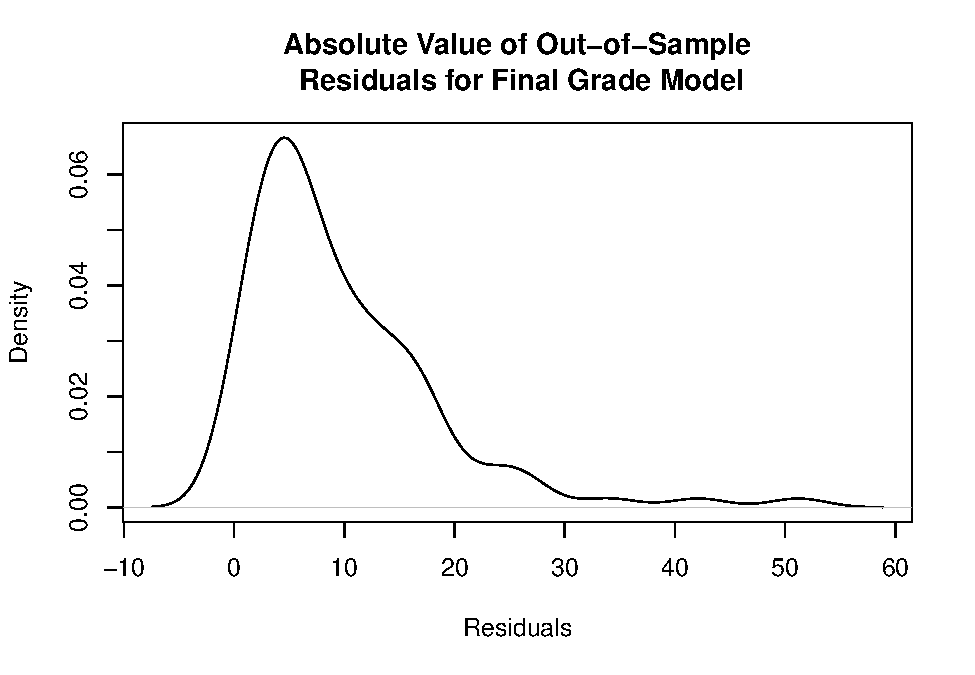
\includegraphics{LAK_Manuscript_files/figure-latex/unnamed-chunk-1-1.pdf}
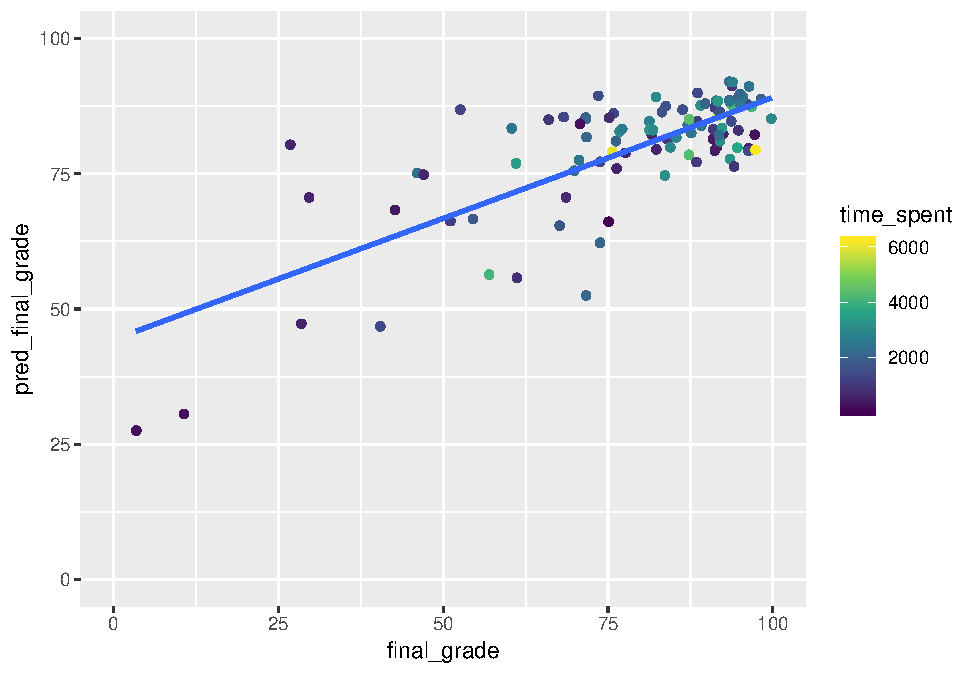
\includegraphics{LAK_Manuscript_files/figure-latex/unnamed-chunk-1-2.pdf}
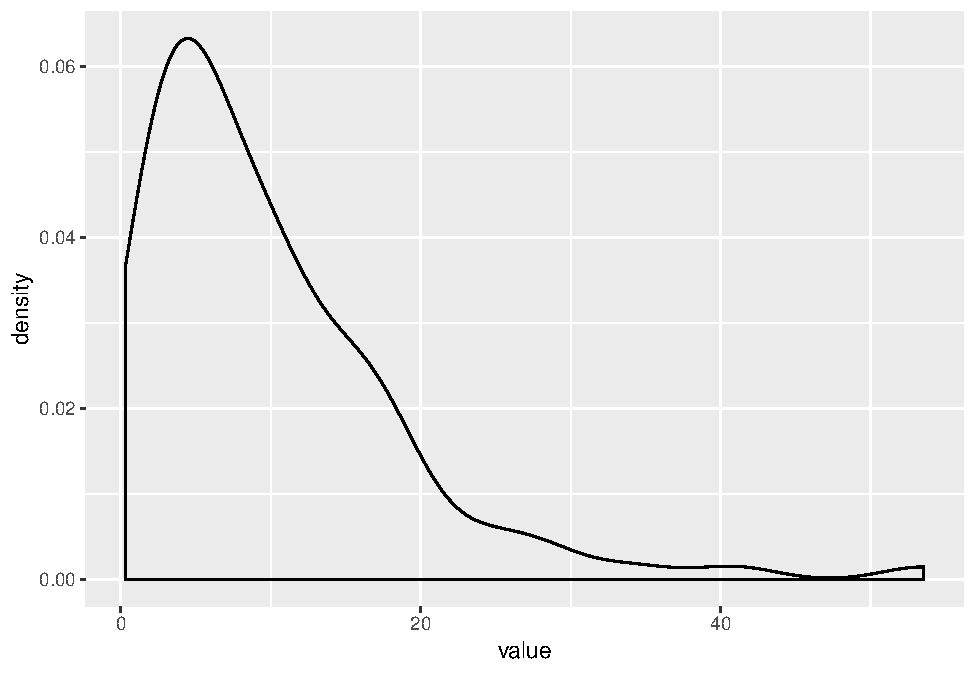
\includegraphics{LAK_Manuscript_files/figure-latex/unnamed-chunk-1-3.pdf}
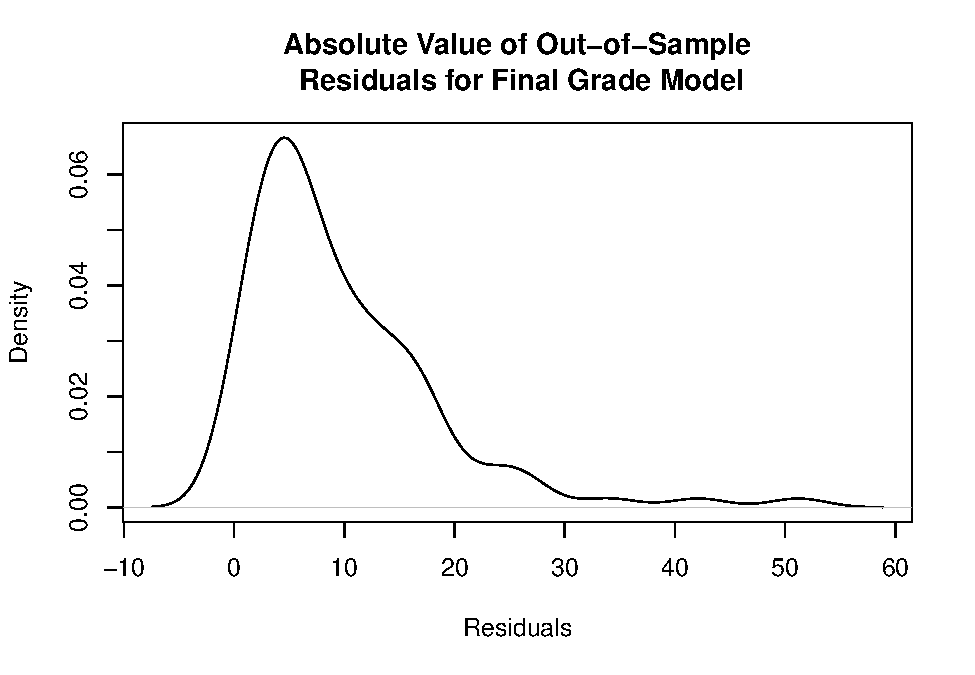
\includegraphics{LAK_Manuscript_files/figure-latex/unnamed-chunk-1-4.pdf}

\begin{verbatim}
## NULL
\end{verbatim}

\begin{figure}
\centering
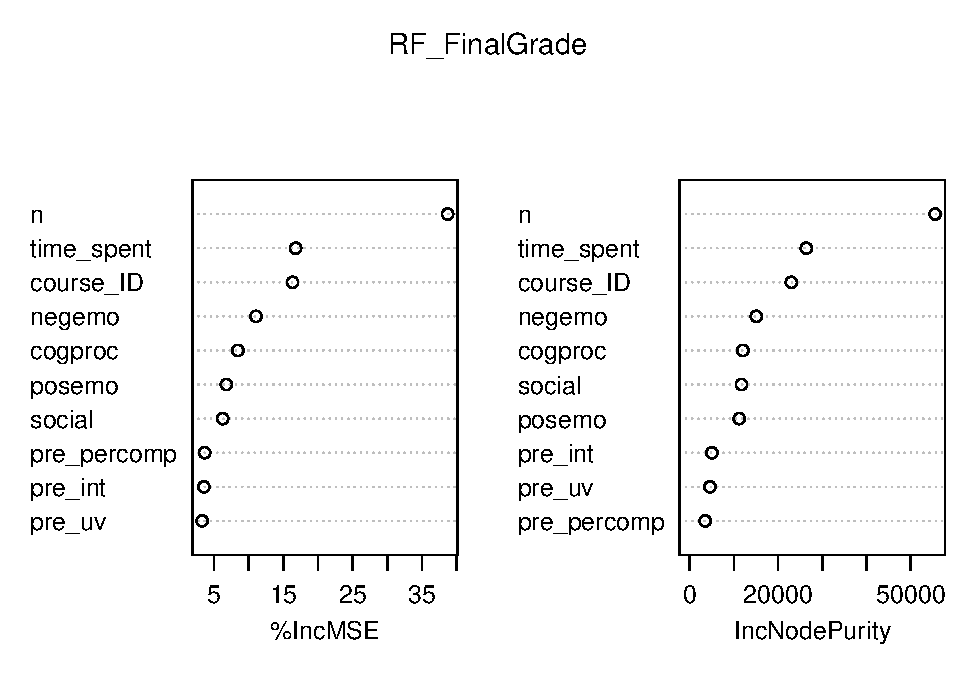
\includegraphics{LAK_Manuscript_files/figure-latex/unnamed-chunk-1-5.pdf}
\caption{}
\end{figure}

\begin{verbatim}
##                      Overall
## pre_int            1.8421541
## pre_uv             3.5007185
## pre_percomp        3.1467335
## time_spent        15.4583594
## enrollment_reason  0.6880564
## course_ID         12.8931753
## cogproc            8.8845678
## social             6.9562230
## posemo             4.4352567
## negemo             8.4379573
## n                 37.1366429
\end{verbatim}

\section{4. DISCUSSION}\label{discussion}

*Below are the specific questions from the LAK website that we should
reflect on\ldots{} maybe not just in the discussion, but also in other
parts of the work as well.

\begin{itemize}
\item
  What is the most surprising part of your results? Was this surprise
  shared by the people involved?
\item
  Can you justify why you used one specific methodology instead of an
  alternative?
\item
  What is the the value and potential impact of your initiative at
  scale?
\item
  What changes in teaching and learning activities you envision that
  could be realistically derived from your work?
\item
  What is the target audience for your study?
\end{itemize}

\newpage

\section{References}\label{references}

\begingroup
\setlength{\parindent}{-0.5in} \setlength{\leftskip}{0.5in}

\hypertarget{refs}{}
\hypertarget{ref-R-papaja}{}
Aust, F., \& Barth, M. (2018). \emph{papaja: Create APA manuscripts with
R Markdown}. Retrieved from \url{https://github.com/crsh/papaja}

\hypertarget{ref-R-base}{}
R Core Team. (2017). \emph{R: A language and environment for statistical
computing}. Vienna, Austria: R Foundation for Statistical Computing.
Retrieved from \url{https://www.R-project.org/}

\endgroup






\end{document}
